\chapter{Linear Algebra}

Welcome to the world of linear algebra, a branch of mathematics that relies on vectors, matrices, and linear transformations. You are familiar with most of these concepts, so in this workbook you’ll see how you can use them together to solve problems.  

Let’s review what you know.

\begin{itemize}
\item \textbf{Vectors}. In workbook 5, you saw how vectors can represent forces and then how to add and multiply them to figure out such things as rocket engine force and direction. 
\item \textbf{Matrices}. In workbook 8 you learned to use spreadsheets to solve problems numerically, like how to figure out the number of barrels a cooper has to produce to achieve a certain take-home pay. Spreadsheets are essentially matrices—a row by column structure that contains values. 
\item \textbf{Linear transformations}. When you studied congruence in workbook 4, you were introduced to a few linear transformations such as translation and reflection. 
\end{itemize}

\section{What's With the Linear?}

You might be thinking, “Hey, haven’t I’ve been doing algebra already?” 

You have. You've come a long way in your problem solving journey. You've used algebra to solve simple equations like $7x + 10 = 24$ and quadratic equations like $4x^{2} + 9x + 31 = 0$. What distinguishes linear algebra is that linear combinations are at its heart. Any equation with a power greater than 1, like a quadratic, is nonlinear.

We’ll first take a look at linear combinations

\section{Linear Combinations}

You won’t see any sin, cos, or tan operations in this section. Linear operations do NOT use trigonometric functions. Those are all nonlinear. A linear combination  preserves addition and scalar multiplication. You will see that linear combinations allow you to solve many types of problems in science and engineering. Before we get deep into the numbers, let’s take a look at a few linear operations you can perform on images. This will give you an intuition for the underlying math. Then we’ll take a look at some numbers.

\section{Image Operations}
The simplest image, a bitmap, can be represented by a two-dimensional matrix of values, either 0, for black, or 1, for white. Grayscale images are also represented by a two-dimensional matrix of values, but the values typically range from 0 to 255. Zero is black, 255 is white, the values in between represent shades of gray. 

Color images are more complex. The simplest color image is a three-dimensional matrix of values. You can think of it as three 2D matrices, one to represent red values (R), another for green values (G), and the third for blue values (B). The combination of R, G, and B determines the color you see.

Working with images, means working with millions of pixels. Fortunately modern techniques make this a snap. Let's look at some common operations on an image of a rocket.

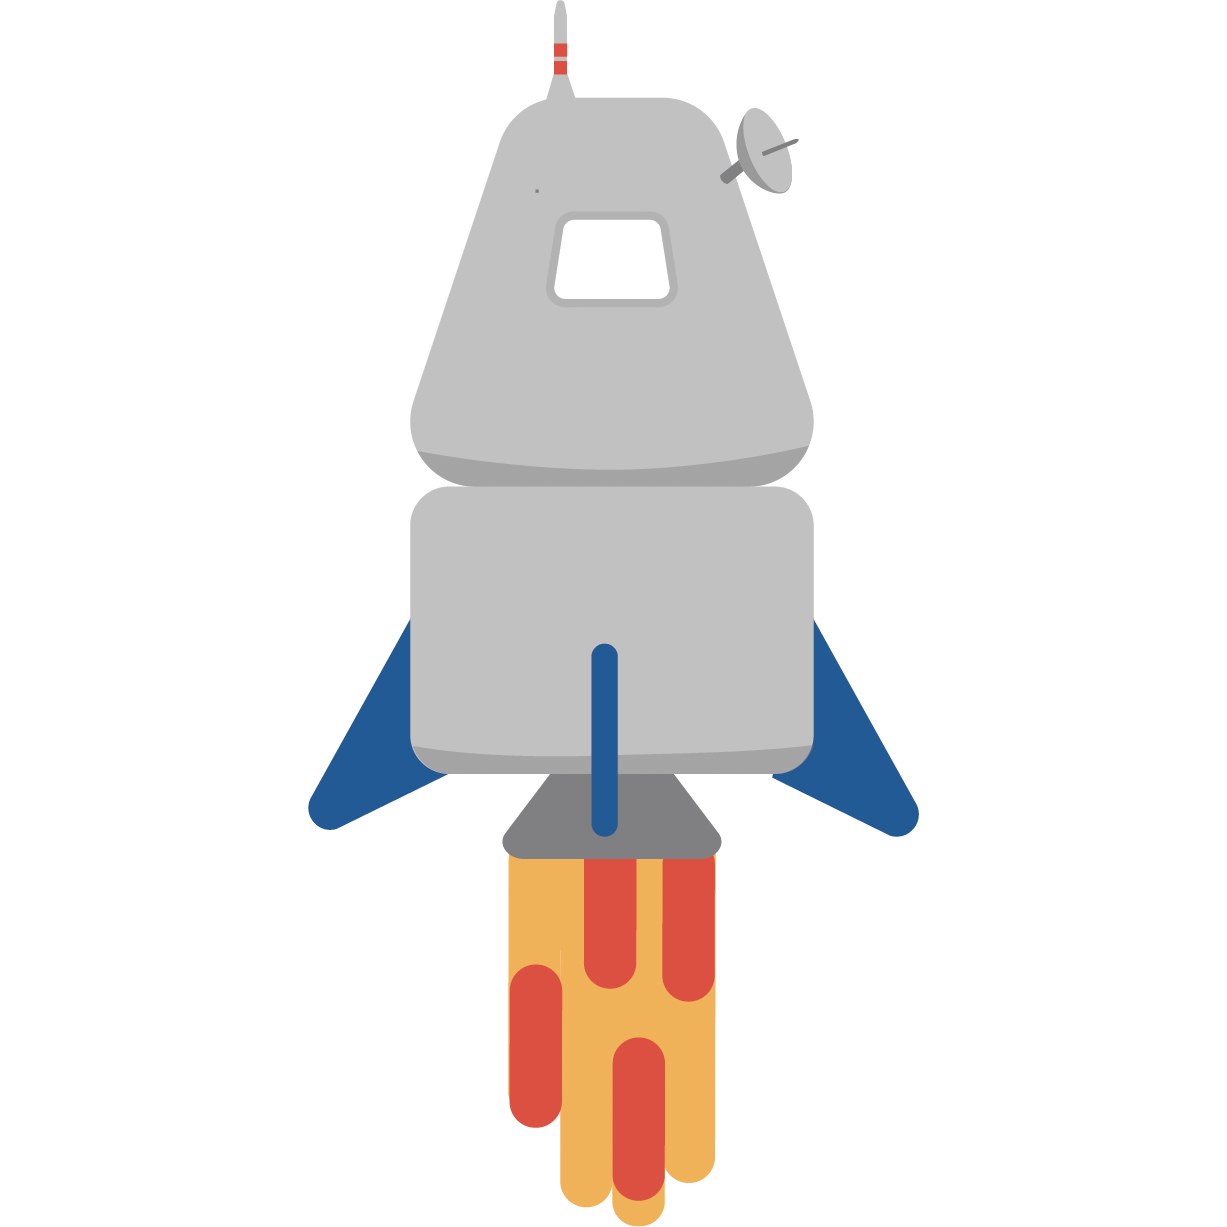
\includegraphics[width=0.25\textwidth]{flying-rocket.png}

Flipping is a linear operation.

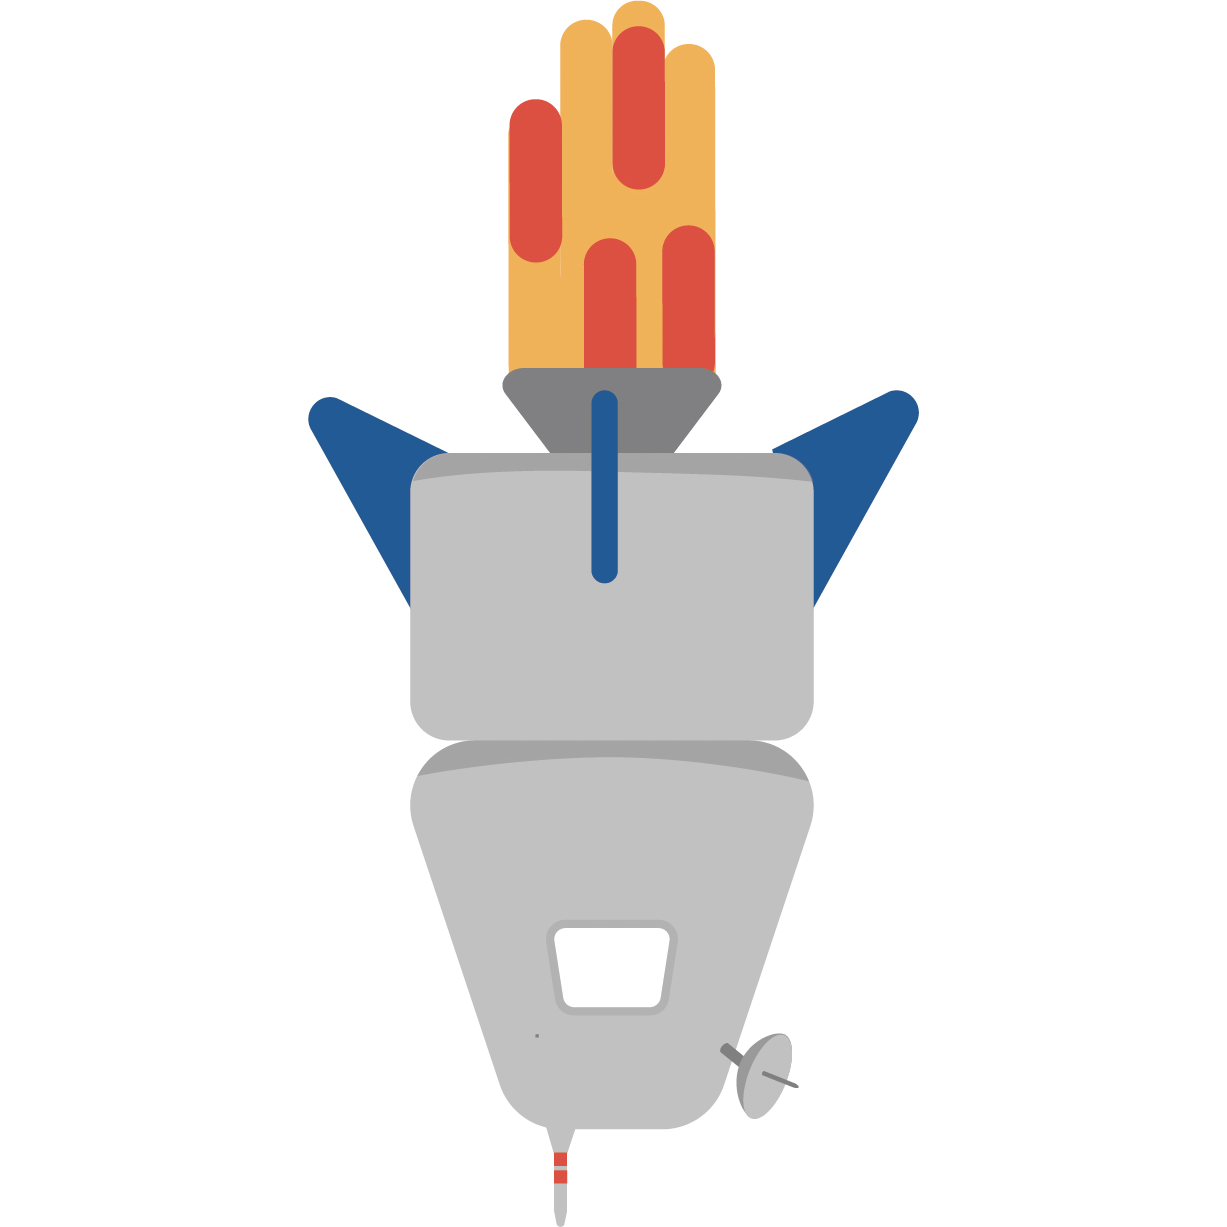
\includegraphics[width=0.25\textwidth]{rocket-flipped.png}

Here it is rotated 90 degrees. This rotation is linear, but if you want to rotate it at an angle that wasn't a multiple of 90, you would need trigonometry. You'd be treading into nonlinear territory. But that happens in the field of linear algebra. You'll learn about nonlinear extensions later that use trigonometric functions and imaginary numbers.

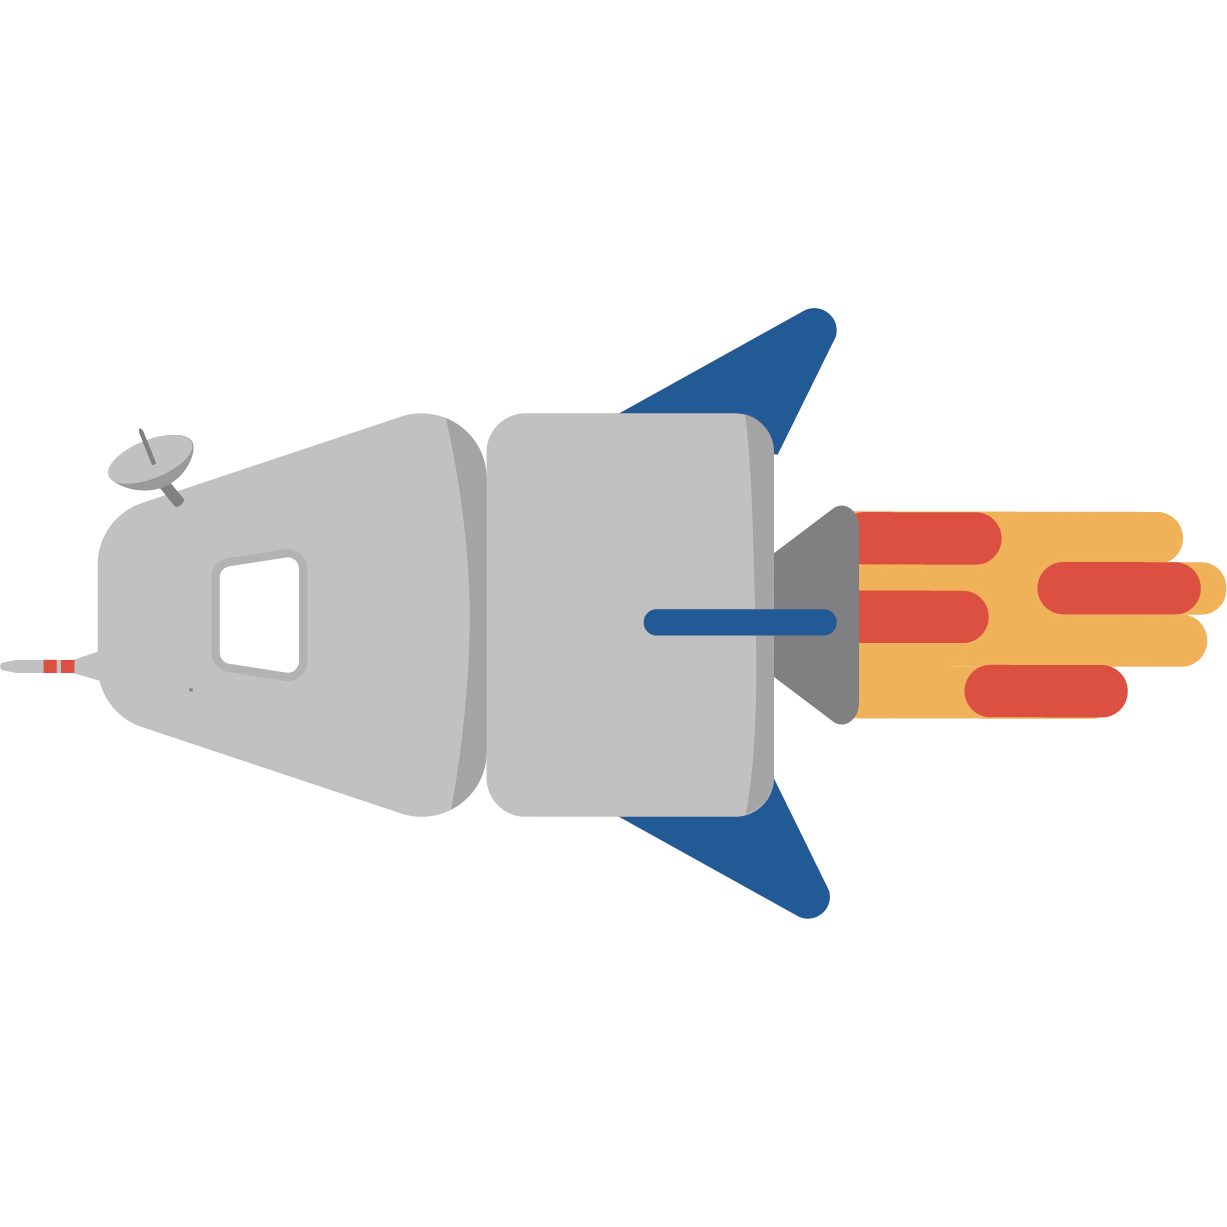
\includegraphics[width=0.25\textwidth]{rocket-rotated-90.png}

Inversion is an interesting linear operation that involves redefining the red, green and blue values such that the new value is 1.0 minus the old value. The resulting black background gives the impression the rocket is in deep space, don't you think?

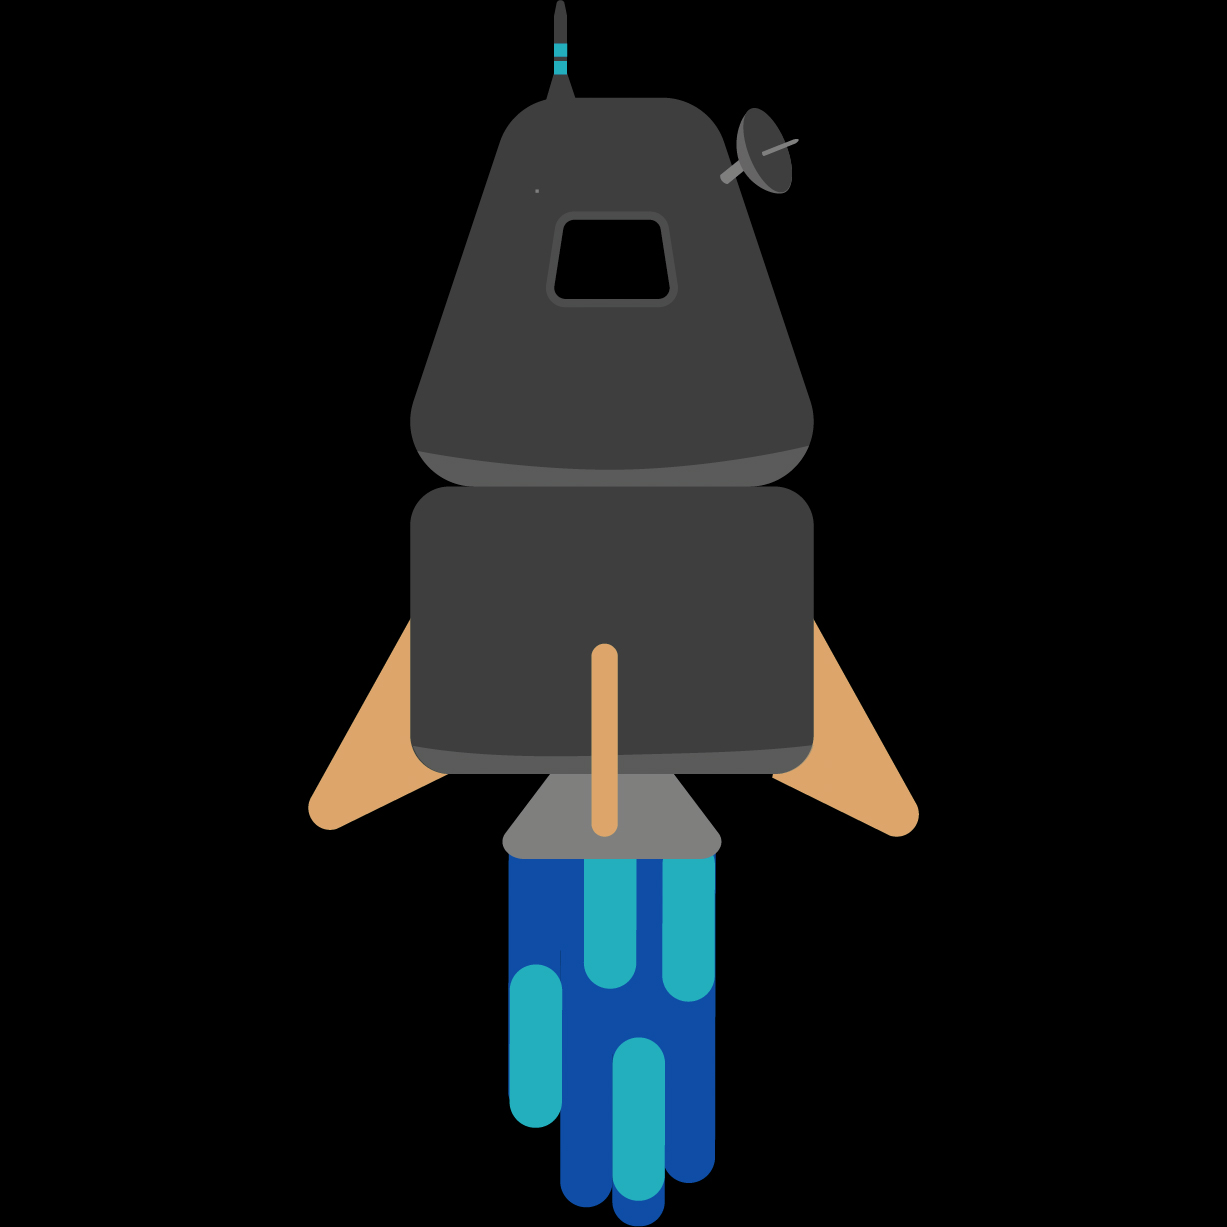
\includegraphics[width=0.25\textwidth]{rocket-inverted.png}

It is possible to redefine the red, green, and blue values in many ways. Visit the NASA website and search for false color images. NASA and other scientists redefine colors to communicate such things as the amount of vegetation or water in an area, the temperatures of the sun's surface, and so on. Photographers often do this for artistic effect. For example, the image on the left was taken with an infrared camera. (But not the thermal infrared you've seen. This is the infrared that's emitted by living plants.) The image is further processed to swap channels. For example, the matrix representing red might be swapped with the matrix representing blue. The image on the right shows the image after swapping color values. All these swapping operations are linear.

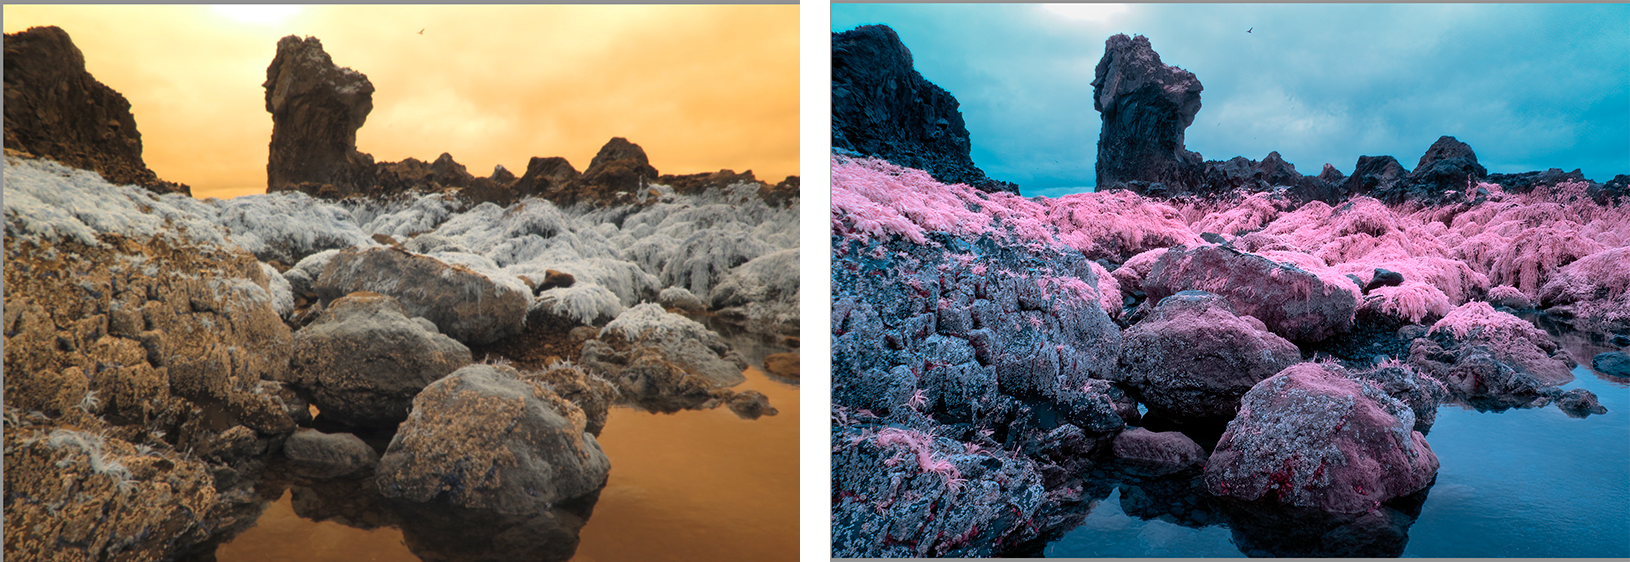
\includegraphics[width=1.0\textwidth]{infrared.png}

\section{The Numbers Behind Some Image Operations}

You'll see a few matrices in this section. Let's first see how a spreadsheet can be represented as a matrix. Recall the barrel making shop example. This is part of that spreadsheet. 

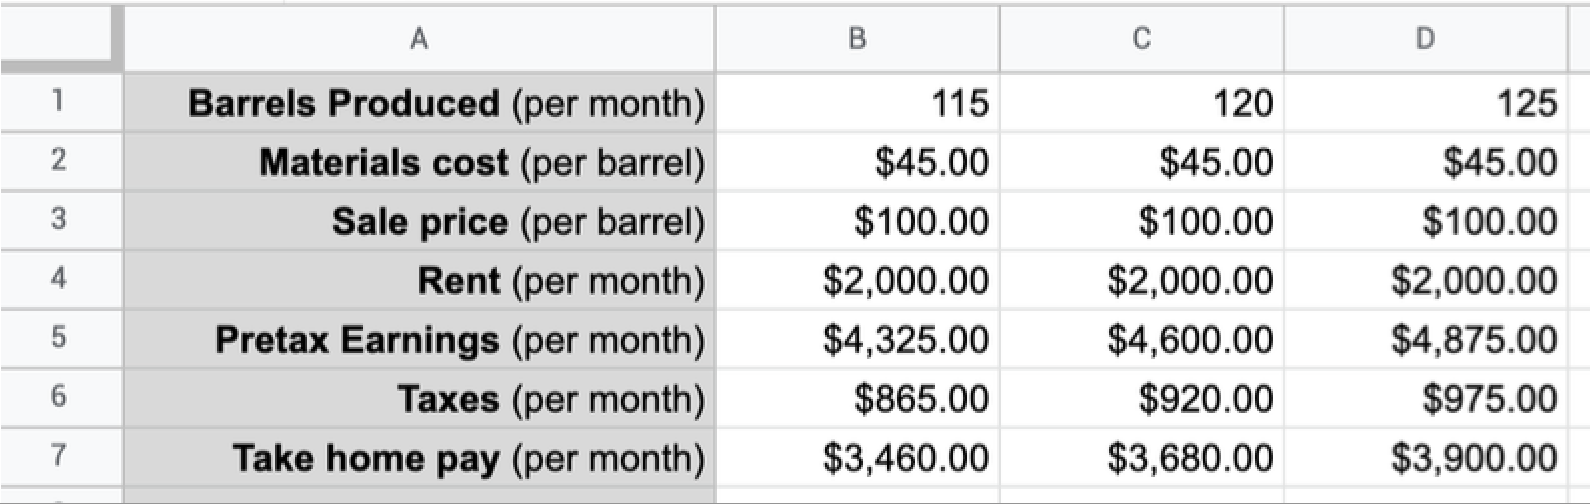
\includegraphics[width=1.0\textwidth]{spreadsheet.png}

Represented as a matrix, it looks like the following. Note the differences. A matrix contains only values, no labels. This matrix uses floating point values, hence the inclusion of decimal points. 

$$\begin{bmatrix}
115. & 120. & 125.\\
45.0 & 45.0 & 45.0\\
100.0 & 100.0 & 100.0\\
2000. & 2000. & 2000.\\
4325. & 4600. & 4875.\\
865. & 920. & 975.\\
3460. & 3680. & 3900.
\end{bmatrix}$$
 
A matrix that represents an image contains only pixel values, whereas the barrel making shop matrix represents seven kinds of variables: barrels produced, materials cost, sales price, rent, pretax earnings, taxes, and take home pay. 

The simplest image to create is a bitmap because that requires a matrix of zeros and ones. This is a matrix for a 10 pixel by 10 pixel image.

$$\begin{bmatrix}
0. & 0. & 0. & 0. & 1. & 0. & 0. & 0. & 1. & 0\\
0. & 0. & 0. & 0. & 1. & 1. & 1. & 1. & 1. & 1\\
0. & 0. & 0. & 0. & 1. & 0. & 0. & 0. & 1. & 0\\
0. & 0. & 0. & 0. & 1. & 0. & 0. & 0. & 1. & 0\\
0. & 0. & 0. & 0. & 1. & 0. & 0. & 0. & 1. & 0\\
0. & 0. & 0. & 0. & 1. & 0. & 0. & 0. & 1. & 0\\
0. & 0. & 0. & 0. & 1. & 0. & 0. & 0. & 1. & 0\\
0. & 0. & 0. & 0. & 1. & 1. & 1. & 1. & 1. & 1\\
0. & 0. & 0. & 0. & 1. & 0. & 0. & 0. & 1. & 0\\
0. & 0. & 0. & 0. & 1. & 0. & 0. & 0. & 1. & 0
\end{bmatrix}$$

When converted to an image, it is very tiny. This is an enlarged version so you can see the pattern.


\includegraphics[width=0.25\textwidth]{normal.png}

We can create an inverse of this image by changing all the values in the matrix so that 0 and 1 and 1 becomes 0. 

$$\begin{bmatrix}
1. & 1. & 1. & 1. & 0. & 1. & 1. & 1. & 0. & 1\\
1. & 1. & 1. & 1. & 0. & 0. & 0. & 0. & 0. & 0\\
1. & 1. & 1. & 1. & 0. & 1. & 1. & 1. & 0. & 1\\
1. & 1. & 1. & 1. & 0. & 1. & 1. & 1. & 0. & 1\\
1. & 1. & 1. & 1. & 0. & 1. & 1. & 1. & 0. & 1\\
1. & 1. & 1. & 1. & 0. & 1. & 1. & 1. & 0. & 1\\
1. & 1. & 1. & 1. & 0. & 1. & 1. & 1. & 0. & 1\\
1. & 1. & 1. & 1. & 0. & 0. & 0. & 0. & 0. & 0\\
1. & 1. & 1. & 1. & 0. & 1. & 1. & 1. & 0. & 1\\
1. & 1. & 1. & 1. & 0. & 1. & 1. & 1. & 0. & 1
\end{bmatrix}$$

When converted to an image and enlarged, it looks like this:

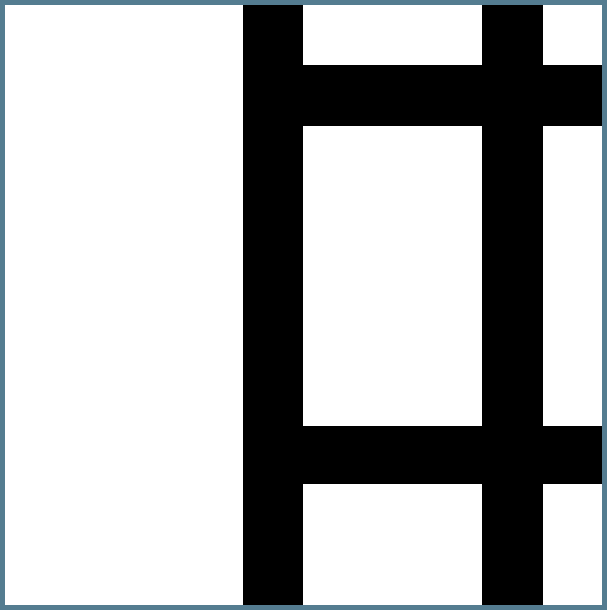
\includegraphics[width=0.25\textwidth]{inverse.png}

Rotating the original matrix by 90 degrees gives this:

$$\begin{bmatrix}
0. & 1. & 0. & 0. & 0. & 0. & 0. & 1. & 0. & 0.\\
1. & 1. & 1. & 1. & 1. & 1. & 1. & 1. & 1. & 1.\\
0. & 1. & 0. & 0. & 0. & 0. & 0. & 1. & 0. & 0.\\
0. & 1. & 0. & 0. & 0. & 0. & 0. & 1. & 0. & 0.\\
0. & 1. & 0. & 0. & 0. & 0. & 0. & 1. & 0. & 0.\\
1. & 1. & 1. & 1. & 1. & 1. & 1. & 1. & 1. & 1.\\
0. & 0. & 0. & 0. & 0. & 0. & 0. & 0. & 0. & 0.\\
0. & 0. & 0. & 0. & 0. & 0. & 0. & 0. & 0. & 0.\\
0. & 0. & 0. & 0. & 0. & 0. & 0. & 0. & 0. & 0.\\
0. & 0. & 0. & 0. & 0. & 0. & 0. & 0. & 0. & 0.
\end{bmatrix}$$

This is the resulting enlarged image:


\includegraphics[width=0.25\textwidth]{rotate90.png}

You'll transpose many matrices in the upcoming pages. It requires swapping rows for columns. 

$$\begin{bmatrix}
0. & 0. & 0. & 0. & 0. & 0. & 0. & 0. & 0. & 0.\\
0. & 0. & 0. & 0. & 0. & 0. & 0. & 0. & 0. & 0.\\
0. & 0. & 0. & 0. & 0. & 0. & 0. & 0. & 0. & 0.\\
0. & 0. & 0. & 0. & 0. & 0. & 0. & 0. & 0. & 0.\\
1. & 1. & 1. & 1. & 1. & 1. & 1. & 1. & 1. & 1.\\
0. & 1. & 0. & 0. & 0. & 0. & 0. & 1. & 0. & 0.\\
0. & 1. & 0. & 0. & 0. & 0. & 0. & 1. & 0. & 0.\\
0. & 1. & 0. & 0. & 0. & 0. & 0. & 1. & 0. & 0.\\
1. & 1. & 1. & 1. & 1. & 1. & 1. & 1. & 1. & 1.\\
0. & 1. & 0. & 0. & 0. & 0. & 0. & 1. & 0. & 0.
\end{bmatrix}$$

The resulting image looks like this:


\includegraphics[width=0.25\textwidth]{transpose.png}

What about adding images? That fits the definition of a linear combination. Recall that grayscale images have values from 0 to 255. To make things simple, let's define two matrices with values ranging from 0.0 to 1.0. When we want a grayscale image, it's easy to multiply the matrix by 255. 

Let's call this matrix f.

$$\begin{bmatrix}
1.0 & 0.5 & 0.0\\
1.0 & 1.0 & 1.0\\
0.5 & 0.0 & 0.0 
\end{bmatrix}$$

When multiplied by 255 and converted to a grayscale image:


\includegraphics[width=0.25\textwidth]{fBitmap.png}

Let's call this matrix g:

$$\begin{bmatrix}
0.5 & 0.0 & 0.0\\
1.0 & 0.5 & 1.0\\
1.0 & 1.0 & 1.0 
\end{bmatrix}$$

When multiplied by 255 and converted to a grayscale image:


\includegraphics[width=0.25\textwidth]{gBitmap.png}

When we add f and g we get k:

$$\begin{bmatrix}
1.5 & 0.5 & 0.0\\
2.0 & 1.5 & 2.0\\
1.5 & 1.0 & 1.0 
\end{bmatrix}$$

But the values in k exceed the range of 0.0 to 1.0, so we normalize by dividing the matrix by 1.0

$$\begin{bmatrix}
0.75 & 0.25 & 0.00\\
1.00 & 0.75 & 1.00\\
0.75 & 0.50 & 0.50  
\end{bmatrix}$$

When multiplied by 255 and converted to grayscale, we get:


\includegraphics[width=0.25\textwidth]{fgBitmapAdded.png}

All the operations we performed on these images satisfy the requirement for linear combinations: preserving addition and scalar multiplication. 

\section{A More Formal Approach}
A linear combination of vectors is the addition of two or more scaled vectors. For example, given two vectors, ${v}_1, {v}_2$ and two scalars $a_1,a_2$, you'd write their linear combination as:

\[x
\mathbf{w} = a_1\mathbf{v}_1 + a_2\mathbf{v}_2
\]

The scalars can be any real number. The vectors can be of any dimension. 

Let's take a more generalized approach. Given vectors $\mathbf{v}_1,
\mathbf{v}_2, ..., \mathbf{v}_n \in \mathbb{R}^m$ and scalars $a_1,
a_2, ..., a_n \in \mathbb{R}$, a linear combination of these vectors
is any vector of the form\index{linear combinations}

\[
\mathbf{w} = a_1\mathbf{v}_1 + a_2\mathbf{v}_2 + ... + a_n\mathbf{v}_n
\]

Each scalar $a_i$ scales the corresponding vector $\mathbf{v}_i$, and
added together, the results are produce a new vector $\mathbf{w}$.

Let's look at an example that has 4 vectors and their scalars. 

$$a_1 = 1, v_1 = [9 1 2]$$
$$a_2 = -1, v_2 = [8 -3 4]$$
$$a_3 = 3, v_3 = [6 0 1]$$
$$a_4 = -4, v_4 = [3 7 2]$$

As a linear combination:

$$\mathbf{w} = 1*[9 1 2] + (-1)*[8 -3 4]+ 3*[6 0 1] + (-4)*[3 7 2]$$

After multiplying each vector by its associated scalar.

$$\mathbf{w} = [9 1 2] + [-8 3 -4] + [18 0 3] + [-12 -28 -8]$$

When combined:

$$\mathbf{w} = [7 -24 -7]$$

\begin{Exercise}[title={Linear Combination}, label=linearCombo]
Calculate the linear combination 
for vectors $v_1, v_2, v_3$ and
scalars $a_1, a_2,a_3$ where:   

$$a1 = 2, v1 = [2 4 8]$$
$$a2 = -2,v2 = [8 -6 3]$$
$$a3 = 4,v3 = [7 9 2]$$

Make sure to show all your work. 
\end{Exercise}
\begin{Answer}[ref=linearCombo]
     \[
	\mathbf{w} = 2*[2 4 8] + (-2)*[8 -6 3] + 4*[7 9 2] 
	\]
  	\[
	\mathbf{w} = [4 8 16] + [-16 12 -6] + [28 36 8] 
	\]  
 	\[
	\mathbf{w} = [16 56 18]  
	\]   
\end{Answer}

\section{Weighted Averages of Vectors}
A weighted average of vectors is a specific type of linear combination
where the coefficients (or weights) $a_i$ are non-negative and sum to
1:\index{weighted averages}
\[
\sum_{i=1}^{n} a_i = 1, \quad a_i \geq 0
\]

A weighted average of vectors $\mathbf{v}_1, \mathbf{v}_2, ...,
\mathbf{v}_n$ is then defined as

\[
\mathbf{w} = a_1\mathbf{v}_1 + a_2\mathbf{v}_2 + ... + a_n\mathbf{v}_n
\]

In this case, each $a_i$ not only scales the corresponding vector
$\mathbf{v}_i$, but also represents the proportion of that vector in
the final average vector $\mathbf{w}$.

Weighted averages are useful when you want to attribute the contribution of one feature or item over another. For example, a teacher might figure a student's final grade using exam scores, class participation, and a final project. The exam scores might make up 65\% of the final grade, class participation 10\%, and a final project 25\%. Thus giving the formula for a grade as:

\[
\mathbf{Grade} = .65*ExamScores + .10*Participation + .25*FinalProject
\]

The teacher defines the weights, making sure they sum to 1.0. 

Let's look at an example where the weights don't sum to 1.0. A store that sells umbrellas might have to get the umbrella stock from three different manufacturers. The store owner buys 100 umbrellas at a cost of \$2.10 each, 50 umbrellas cost \$1.85 each, and 200 umbrellas cost \$2.00. 

\[
\mathbf{TotalCost} = 2.10*100 + 1.85*50 + 2.00*200 = 702.5
\]

To calculate the weighted average, divide the total cost by the number of items.

\[
\mathbf{WeightedAverage} = 702.5/350 = 2.01 
\]

\begin{Exercise}[title={Weighted Average}, label=weightedAverage]
A concert sells 300 tickets in the balcony at \$50 each, 100 tickets on the main floor at \$75 each, and 50 tickets in the section closest to the stage at \$150 each. What's the weighted average?
\end{Exercise}
\begin{Answer}[ref=weightedAverage]
\[\mathbf{TotalSales} = 50*300 + 75*100 + 150*50 = 30,000\]
\[\mathbf{NumberTickets} = 300 + 100 + 50 = 450\]
\[\mathbf{WeightedAverage} = 30,000/450 = 66.67\]
\end{Answer}

\section{Weighted Averages of Vectors in Python}
Create a file called \filename{linearCombos.py} and enter this code:

\begin{Verbatim}
// import the python module that supports matrices
import numpy as np

// an array for number of umbrellas by manufacturer
items = np.array([100, 50, 200])

// weights are the cost of item by manufacturer
weights = np.array([2.10, 1.85, 2.00])

// create an array for total cost for each manufacturer
costPerManufacturer=items * weights

// sum the individuals costs to get the total
totalCost = np.sum(costPerManufacturer)

// get number of items
numItems = np.sum(items) 

// you are ready to calculated the weighted average
weightedAverage = totalCost/numItems
print(weightedAverage)
\end{Verbatim}

When you run this code, you should get a weighted average of \$2.01 when rounded to the nearest cent.


